\subsubsection{Subsystem Overview}
The computing platform's power subsystem consists of an integrated battery and power management pack purchased commercially. The devices powered by this system are the following:

\begin{itemize}
\item Platform Management Board (Raspberry Pi) -- maximum current draw of 0.5 A and a typical current draw of 0.4 A, and
\item Programmable Logic Board (Zedboard) -- maximum current draw of 1 A and a typical current draw of 0.4 A
\end{itemize}

The power system must provide continuous power to the computing platform for at least 20 minutes (\textbf{F.PR.1}).

\subsubsection{Seperate vs Common Power Supplies}
When designing the power system we had to choose between having a common power supply for the both the drone itself as well as the computational hardware or to have seperate power supplies. The relative advantages and disadvantages of these options are as follows.

\textbf{Seperate Power Supplies}:
\begin{itemize}
    \item No risk of noise from the motors interfering with the computational hardware.
    \item Allows for testing of the computational hardware seperately from the drone.
    \item More easily allows us to upgrade to another drone if neccesary.
    \item Ultimately results in more weight than if we had had a single power supply.
    \item Having to buy a second battery results in slightly more cost than a common power supply.
\end{itemize}

The pros and cons of a common power supply are largely the inverse of the above. Ultimately we decided that the advantages of using separate power supplies, in particular not having to worry about noise from the motors and the extra flexibility we would have when testing, outweighed the disadvantages.

\subsubsection{SRAD vs COTS Power Supply}
We had initially planned on using an SRAD power supply system. It was to consist of a lithium-polymer or lithiumi-ion battery and a battery management system. The battery management system (seen in Figure \ref{powerdiag}) would have consisted of two DC-DC converters(efficiency ~94%), a battery protection board, and a battery monitor. 

\begin{figure}[H]
\centering
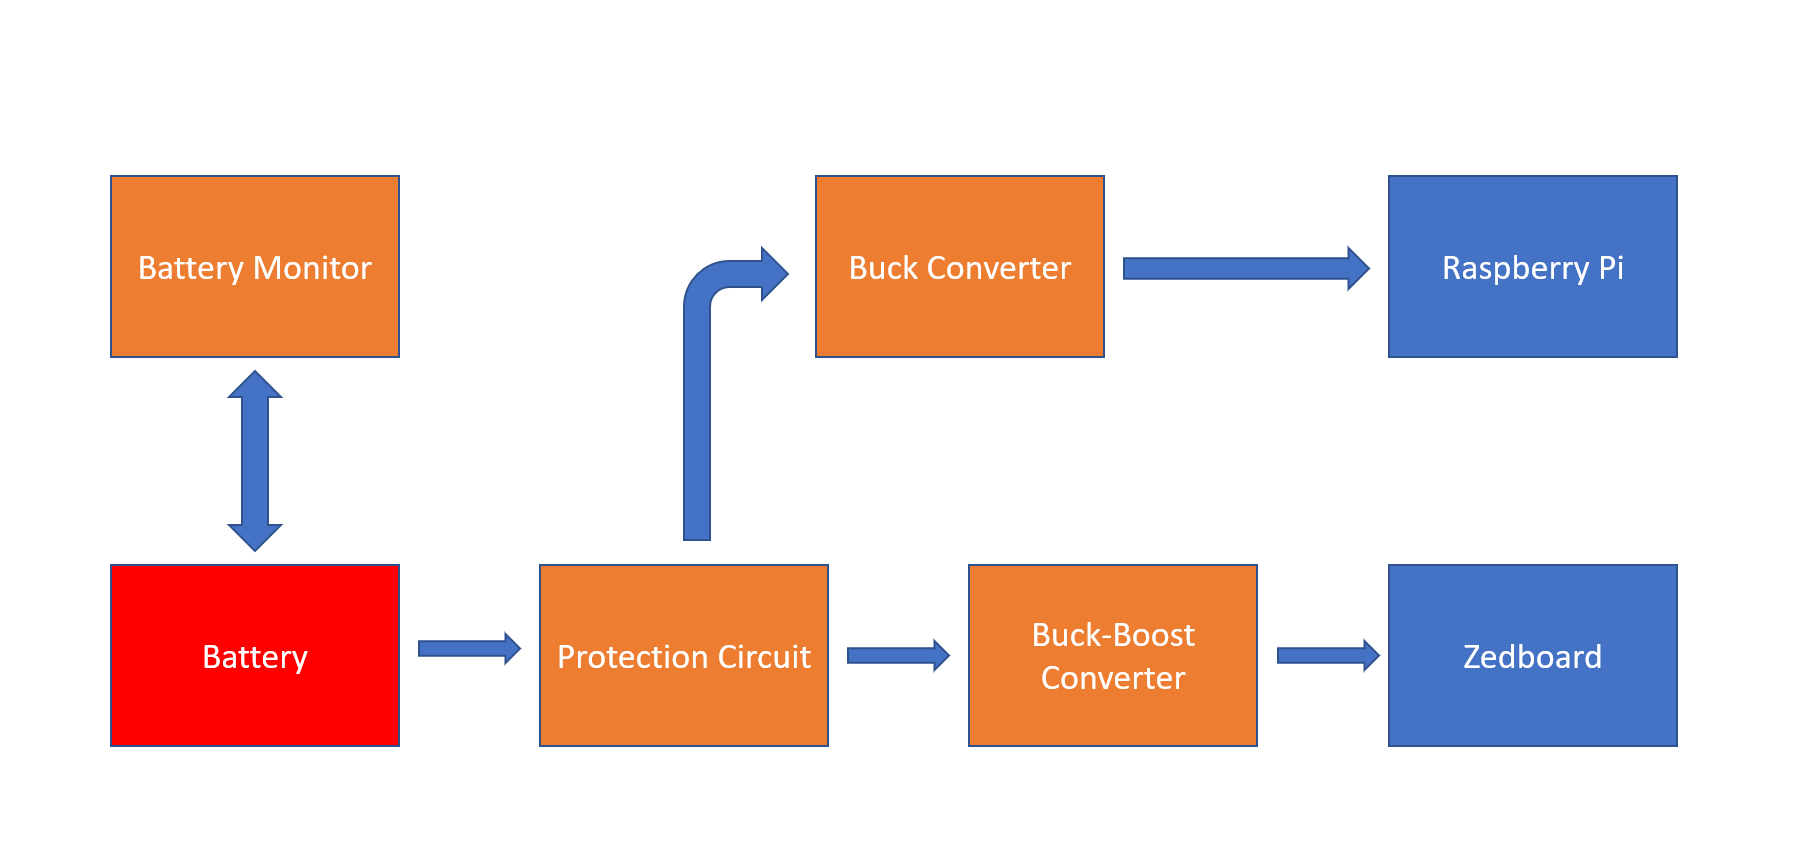
\includegraphics[width=15cm]{img/Power_Diagram.png}
\caption{Computing Platform Power Subsystem}
\label{powerdiag}
\end{figure}

DC-DC conversion would have been accomplished using a buck converter for the 5 V output and a buck-boost converter for the 12 V output. 

The battery protection board was to consist of a Zener diode to provide undercurrent protection, a fuse to provide overcurrent protection, and a simple circuit to provide reverse polarity protection (\textbf{F.PR.4-6}). Reverse polarity protection would additionally have been achieved by using connectors that cannot be connected in reverse (\textbf{F.PR.6}). 

After designing this system a COTS system was found that fits our requirements. The COTS system consists of 3 lithium-ion batteries with a combined capacity of 3000mAh and a power management circuit inside a plastic case. The plastic case has a 5V USB output and a 12V output that are compatible with the Raspberry Pi and the Zedboard respectively. The rated current output of 3A is high enought to supply both of the boards at the same time and the plastic case can even be removed to reduce weight if this is deemed necessary.

The SRAD system was scrapped in favor of the COTS system. The cots system provides all of the functionality of the SRAD system at a lower cost and in a smaller form factor. As designing a power system is not the goal of this project we decided that with an available COTS solution it did not make sense to continue with the SRAD system.

\subsubsection{Battery}
The power subsystem utilizes Lithium-ion batteries integrated with a power management circuit in a single package. In order to
power the computing system for 20 minutes the battery will need to have a capacity of 233mAh. Since that is a non-standard size, as well as to allow for multiple uses without recharging the battery pack that we are using has a capacity of 3000mAh. This should provide 3 hours and 45 minutes of operation.

